\documentclass[aspectratio=169]{beamer}
\usepackage[latte]{catppuccinpalette}
\usepackage{booktabs}
\usepackage{graphicx}
\setbeamercolor{structure}{fg=CatLatteTeal}
\setbeamercolor{title}{fg=CatLatteTeal}
\setbeamercolor{frametitle}{fg=CatLatteTeal}
\setbeamertemplate{navigation symbols}{}
\title{NetSy: Network Emissions Synthesizer}
\date{}
\newcommand{\SeedNote}{NetSy seeds 1--3; one fixed MASS-GT reference. Ranges show seed sensitivity, not confidence intervals or a formal equivalence test.}
\newcommand{\ActorTable}{\centering\small\begin{tabular}{lrr}\toprule Indicator & MASS-GT & NetSy\\\midrule Actors retained & 86\,004 & 84\,532--85\,849\\ Size retained (jobs) & 1\,034\,015 & 1\,033\,511--1\,039\,856\\ SIF: max. error after rounding & \multicolumn{2}{c}{0.000 tonnes/year}\\ \bottomrule\end{tabular}\par}
\newcommand{\FreightTable}{\centering\small\begin{tabular}{lrr}\toprule Indicator & MASS-GT & NetSy\\\midrule Shipments & 118\,961 & 118\,345--118\,637\\ Daily shipment tonnes & 401\,438.24 & 401\,438.24\\ Freight tours & 60\,062 & 59\,802--60\,271\\ Freight VKT (million) & 20.907 & 20.878--21.091\\ \bottomrule\end{tabular}\par}
\newcommand{\ParcelVanTable}{\centering\small\begin{tabular}{lrr}\toprule Indicator & MASS-GT & NetSy\\\midrule Customer parcels/day & 228\,707 & 228\,707\\ Service van trips/day & 367\,479.1 & 367\,497.9\\ Construction van trips/day & 178\,228.8 & 178\,247.0\\ Max. OD-cell difference & -- & 0.008 trips\\ \bottomrule\end{tabular}\par}
\newcommand{\SavingsText}{Savings vs. the corrected port: \textbf{10.2\% less VKT}, with +3.8\% tours. Same 228\,707 customer parcels.}
\newcommand{\AssignmentTable}{\centering\small\begin{tabular}{lrr}\toprule Indicator & MASS-GT & NetSy\\\midrule Network links compared & \multicolumn{2}{c}{158\,806}\\ Max. connector trip error & -- & 8.467\\ Max. non-connector trip error & -- & 0.000020\\ CO$_2$ (tonnes/day) & 16\,792.874 & 16\,795.387\\ CO$_2$ change explained by fix & \multicolumn{2}{c}{2.513 tonnes/day}\\ \bottomrule\end{tabular}\par}
\newcommand{\AssignmentNote}{CO$_2$ residual after accounting for the fix: 0.248 g. Small load residuals occur on connectors (ties and the reference's eight-neighbour link lookup); see the audit.}
\newcommand{\UccTable}{\centering\small\begin{tabular}{lrr}\toprule Indicator & MASS-GT UCC & NetSy UCC + pooling\\\midrule Freight tours & 62\,931 & 62\,709\\ Parcel tours & 1\,760 & 1\,505\\ Customer parcels & 228\,707 & 228\,707\\ Network VKT (million) & 44.078 & 43.925\\ CO$_2$ (tonnes/day) & 16\,761.0 & 16\,712.0\\ \bottomrule\end{tabular}\par}
\newcommand{\UccNote}{Independent stochastic runs, documented fixes and explicit outbound hub pooling; this is a scenario comparison, not an exact-match claim. Reference repaired only for execution/midnight handling; behavioural bugs are listed in the audit.}
\newcommand{\MicroTable}{\centering\small\begin{tabular}{lrr}\toprule Indicator & MASS-GT (corrected) & NetSy\\\midrule Hub-bound customer parcels & 7\,208 & 7\,208\\ Max. hub--recipient pair error & -- & 0\\ Customer parcels delivered & \multicolumn{2}{c}{228\,707}\\ Completed parcel tours & No hub-aware schedule & 1\,811\\ \bottomrule\end{tabular}\par}
\newcommand{\MicroNote}{Collaborative electric-bicycle configuration from the supplied Dutch microhub tables. Raw-reference maximum hub-pair difference: 391 parcels; corrected difference: zero. Both references are retained; zero pair error is against corrected selection. NetSy adds the missing hub-aware downstream operations.}
\newcommand{\CopertText}{Full pipeline, same seed-1 trips:\par factors: 16\,768.2 t CO$_2$;\par COPERT: 18\,140.3 t CO$_2$.\par\medskip A model/fleet sensitivity, not a measured emissions improvement.}
\newcommand{\CopertNote}{Declared Euro VI truck / Euro 6 van fleet; EMEP/EEA Appendix 4 (July 2026). Curve: medium truck, 0\% grade, 50\% payload. Dutch network run assumes flat grades; no non-exhaust estimate is claimed. Paper informs the speed/grade/payload and hub/powertrain extension.}
\newcommand{\BrowserText}{ The 6\,089\,837-row loads file loaded in 2.1 s in the recorded browser check.}
\newcommand{\ValidationSummary}{three NetSy seeds assess stochastic sensitivity, and original-trip controls isolate assignment/emissions.}
\newcommand{\BoundaryNote}{Scope: the standard Dutch pipeline, UCC and collaborative microhub case. Optional crowdshipping and selected-link analyses are not benchmarked here. Benchmark agreement is distinct from empirical validity of a new study case. Code, patches, inputs and comparison scripts are identified in validation/.}

\begin{document}

\begin{frame}{NetSy: Network Emissions Synthesizer}
\begin{itemize}
\item Generalize MASS-GT for different study cases: the same mechanisms, with local evidence and classifications supplied as data.
\item Preserve a comparable pipeline: actors, flows, shipments, tours, road loads and emissions.
\item Add modelling contributions, including COPERT V emissions informed by Dias \& Jenelius (2026).
\end{itemize}
\vfill
\footnotesize Comparisons below use MASS-GT's own Dutch study-area data.\par
\scriptsize Paper: \href{https://doi.org/10.1016/j.ubtr.2026.100031}{Urban Transitions 5, 100031}.
\end{frame}

\begin{frame}{Actors and commodity flows: port + generalization}
\ActorTable
\medskip
\begin{itemize}
\item Firms become agents of any class; jobs become general stratum-size totals.
\item SIF's regressions and FRATAR operate on supplied attributes, resources and regions.
\end{itemize}
\vfill\scriptsize\SeedNote
\end{frame}

\begin{frame}{Shipments and freight tours: port + generalization}
\FreightTable
\medskip
\begin{itemize}
\item Keep sourcing, shipment-size/vehicle choice, delivery windows and end-tour logits.
\item Replace Dutch categories with resource/segment strata and typed facilities.
\end{itemize}
\vfill\scriptsize\SeedNote
\end{frame}

\begin{frame}{Parcel demand and service vans: port + generalization}
\ParcelVanTable
\medskip
\begin{itemize}
\item Same parcel-demand mechanism; population strata and operators are data.
\item Service/construction gravity models share a general matrix-balancing core.
\end{itemize}
\vfill\scriptsize Van comparison uses all OD cells; small numerical differences are retained, not labelled exact matches.
\end{frame}

\begin{frame}{Parcel routes: separate the fix from the contribution}
\begin{columns}
\column{.62\textwidth}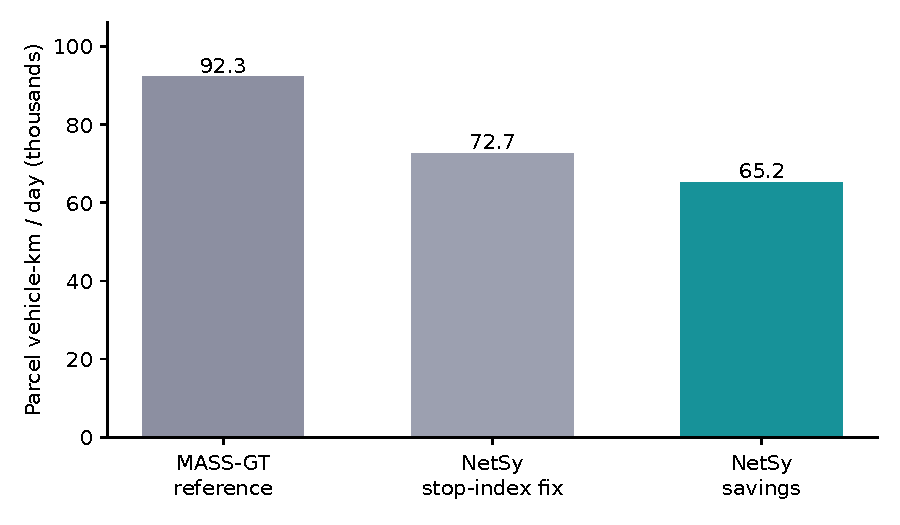
\includegraphics[width=\linewidth]{figures/parcels.pdf}
\column{.36\textwidth}
\small
\textbf{Fix:} use the actual next zone when ordering stops.\par\medskip
\textbf{Contribution:} Clarke--Wright savings and stop relocation.\par\medskip
\SavingsText
\end{columns}
\vfill\scriptsize Same demand, capacity and Dutch skims; VKT from the zone-to-zone skim, including returns.
\end{frame}

\begin{frame}{Assignment and factors: controlled comparison}
\AssignmentTable
\medskip
\begin{itemize}
\item Supply MASS-GT's original trips to both assignments: isolate this stage from synthesis randomness.
\item Fix urban parcel emissions being overwritten instead of accumulated.
\end{itemize}
\vfill\scriptsize\AssignmentNote
\end{frame}

\begin{frame}{UCC scenario: port, fixes and hub pooling}
\UccTable
\medskip
\small
Explicit facility legs and carriers; vehicle/combustion choices; electric and hybrid operations. NetSy additionally pools outbound parcels at each hub.\par\medskip
Vehicle shares are counted once per vehicle, with an explicit fuel fallback. Midnight matrix generation and the reference's single-worker hybrid dispatch are repaired.
\vfill\scriptsize\UccNote
\end{frame}

\begin{frame}{Microhubs: preserve the model, complete its operations}
\MicroTable
\medskip
\small
\textbf{Port + fixes:} hub selection and two parcel legs; correct selected-hub IDs and zone indexing.\par\medskip
\textbf{Downstream extension:} hub-based collaborative tours with vehicle-specific capacity, speed and powertrain.
\vfill\scriptsize\MicroNote
\end{frame}

\begin{frame}{COPERT V: an additional emissions model}
\begin{columns}
\column{.60\textwidth}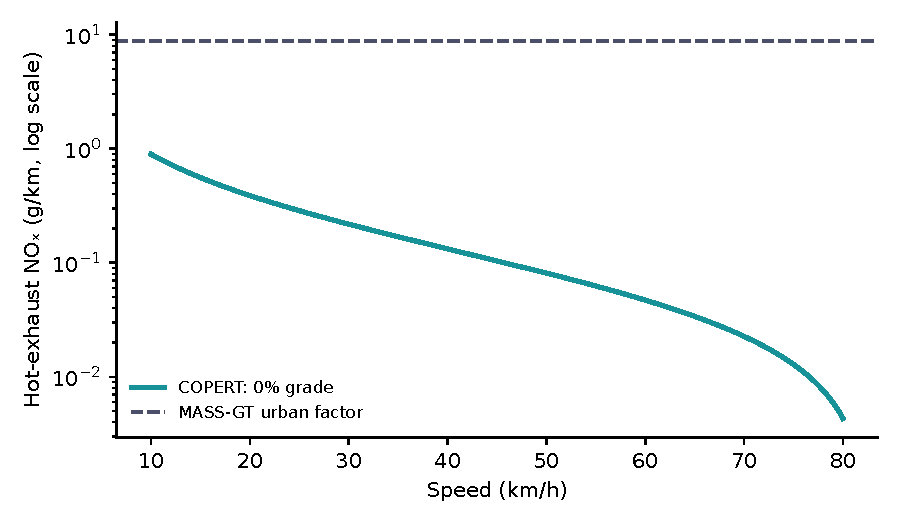
\includegraphics[width=\linewidth]{figures/copert.pdf}
\column{.38\textwidth}\small
Speed, grade and payload select hot-exhaust factors. Keep payload bins separate before aggregation.\par\medskip
\CopertText
\end{columns}
\vfill\scriptsize\CopertNote
\end{frame}

\begin{frame}{Implementation improvements and validation boundary}
\small
\begin{itemize}
\item Array bookkeeping, cached proximity and compiled stop improvement; preserve the baseline tour result.
\item Parquet outputs and column-based browser tables.\BrowserText
\item Stage comparisons separate inherited behaviour, generalization, fixes and modelling additions; \ValidationSummary
\end{itemize}
\vfill\scriptsize\BoundaryNote
\end{frame}
\end{document}
